\chapter[Conclusão]{Conclusão}

Este capítulo apresenta a síntese das atividades realizadas ao longo da monografia, retoma os objetivos definidos para 
o trabalho e discute os principais resultados obtidos com a execução do experimento.

\section{Atividades Propostas}

A Tabela~\ref{tab:atividades_conclusao} apresenta a situação das atividades previstas ao longo da monografia, 
contemplando tanto as atividades desenvolvidas no TCC 1 quanto aquelas executadas no TCC 2. A primeira etapa 
concentrou-se na construção do referencial teórico, na revisão da literatura e no planejamento experimental. 
A segunda etapa contemplou a preparação da base, a execução dos tratamentos, a consolidação dos dados, a análise 
estatística e a redação final dos resultados.

\begin{table}[h!]
\centering
\caption{Situação das atividades da monografia}
\label{tab:atividades_conclusao}
\begin{tabular}{lcc}
\hline
\textbf{Atividade} & \textbf{Etapa} & \textbf{Situação} \\
\hline
Contextualização sobre Garantia de Qualidade e \textit{Code Smells} & TCC 1 & Concluída \\
Definição do GQM & TCC 1 & Concluída \\
Elaboração do protocolo da Revisão Estruturada da Literatura & TCC 1 & Concluída \\
Seleção dos artigos & TCC 1 & Concluída \\
Leitura do material selecionado & TCC 1 & Concluída \\
Definição da proposta de solução & TCC 1 & Concluída \\
Redação da primeira versão da monografia & TCC 1 & Concluída \\
Revisão & TCC 1 & Concluída \\
Apresentação da primeira etapa & TCC 1 & Concluída \\
\hline
Evolução e ajustes do trabalho & TCC 2 & Concluída \\
Preparação e coleta dos dados & TCC 2 & Concluída \\
Análise dos dados & TCC 2 & Concluída \\
Documentação dos resultados & TCC 2 & Concluída \\
Redação final da monografia & TCC 2 & Concluída \\
Revisão final & TCC 2 & Concluída \\
Apresentação final & TCC 2 & Agendada \\
\hline
\end{tabular}
\end{table}

Durante a execução do TCC 2, algumas dessas atividades foram desdobradas em subatividades, necessárias para viabilizar a condução do experimento. 
A atividade de preparação e coleta dos dados, por exemplo, envolveu o tratamento do dataset, a reconstrução dos trechos de código, configuração do ambiente e execução do experimento. 
De forma semelhante, a análise dos dados incluiu etapas específicas de análise estatística e análise descritiva. 
Esses desdobramentos permitiram acompanhar a execução do trabalho de forma mais detalhada, mantendo a tabela final organizada em atividades principais.

\section{Resultados Obtidos}

Os resultados obtidos ao longo deste trabalho podem ser organizados em duas dimensões principais. A primeira corresponde ao 
embasamento teórico e metodológico construído a partir da síntese da literatura relacionada e no planejamento experimental. A segunda corresponde aos resultados 
empíricos obtidos com a execução do experimento comparando SonarQube e modelos de linguagem na detecção de \textit{code smells}.

Na etapa inicial, os artigos analisados evidenciaram que ferramentas de análise estática, como o SonarQube, continuam amplamente 
utilizadas na indústria devido à sua eficiência, integração com pipelines de desenvolvimento e capacidade de aplicar regras 
automatizadas sobre o código-fonte. No entanto, a literatura também aponta limitações dessas ferramentas, como a dependência de 
limiares fixos, a geração de falsos positivos e a dificuldade em capturar aspectos semânticos mais complexos do código.

Em paralelo, observou-se um crescimento de pesquisas que investigam o potencial da Inteligência artificial
em tarefas de compreensão e avaliação de código. Diversos estudos apontam que abordagens envolvendo IA e Machine Learning conseguem
identificar padrões estruturais e semânticos que extrapolam as regras tradicionais de análise estática, abrindo espaço
para novas possibilidades em detecção de code smells, previsão de defeitos, explicações automáticas e
refatorações sugeridas. Apesar disso, as pesquisas também apontam desafios relevantes, como a falta de padronização
das respostas dos modelos, o risco de alucinações, a dificuldade de controlar variações entre versões e a necessidade
de protocolos rigorosos de avaliação empírica.

A revisão estruturada também evidenciou uma lacuna relevante: embora existam estudos sobre ferramentas tradicionais e estudos 
sobre modelos baseados em IA, ainda são menos frequentes comparações experimentais diretas entre ferramentas de análise estática 
e LLMs para detecção de \textit{code smells}. Essa lacuna fundamentou a proposta experimental deste trabalho.

Na etapa experimental, foram avaliados sete tratamentos: SonarQube, ChatGPT zero-shot, ChatGPT few-shot, Claude zero-shot, 
Claude few-shot, DeepSeek zero-shot e DeepSeek few-shot. A unidade de análise foi definida como o par \texttt{sample\_id} e 
\texttt{smell}, considerando que um mesmo trecho de código pode ser avaliado em relação a mais de um \textit{code smell}. 
Os resultados dos tratamentos foram comparados ao \textit{ground truth} do MLCQ, e cada predição foi codificada como acerto 
ou erro em relação ao veredito de referência.

A análise estatística principal teve como objetivo verificar se havia diferença significativa entre as proporções de acerto 
dos tratamentos. Como os dados são binários e pareados, foi aplicado o teste de Cochran's Q. O resultado indicou rejeição da 
hipótese nula, com $Q = 886{,}96$ e $p$-valor igual a $2{,}47 \times 10^{-188}$. Assim, conclui-se que há evidência estatística 
de diferença entre os tratamentos avaliados. O coeficiente $W$ de Kendall foi igual a 0,01697, indicando que, embora a diferença 
seja estatisticamente significativa, o tamanho de efeito global é baixo.

Após o teste global, foram realizadas comparações par a par com o teste de McNemar, aplicando-se a correção de Holm-Bonferroni 
para controle do erro Tipo I acumulado. Das 21 comparações realizadas, 19 apresentaram diferença estatisticamente significativa 
após a correção. Apenas os pares ChatGPT few-shot versus Claude zero-shot e ChatGPT zero-shot versus DeepSeek zero-shot não 
apresentaram diferença significativa. Esses resultados confirmam que, na maior parte das comparações, os tratamentos apresentaram 
comportamentos distintos em relação à proporção de acerto.

Na análise geral por tratamento, o SonarQube apresentou a maior taxa de acerto, com valor aproximado de 0,897. Entre as LLMs, o 
melhor resultado nessa métrica foi obtido pelo DeepSeek few-shot, com taxa de acerto aproximada de 0,888. Em seguida, apareceram 
ChatGPT zero-shot e DeepSeek zero-shot, com taxas de acerto próximas de 0,880. No entanto, a taxa de acerto geral deve ser 
interpretada com cautela, pois a base apresenta predominância de casos negativos, isto é, casos em que o MLCQ indica ausência de \textit{smell}.

As métricas de classificação mostraram diferenças importantes entre os tratamentos. O SonarQube apresentou alta especificidade, 
com valor aproximado de 0,974, indicando boa capacidade de reconhecer corretamente casos negativos. Entretanto, apresentou baixo 
\textit{recall}, com valor aproximado de 0,264, o que indica que deixou de identificar parte relevante dos casos positivos. 
Esse comportamento caracteriza uma abordagem mais conservadora.

As LLMs, por outro lado, apresentaram maior tendência a predizer a presença de \textit{smells}. Esse comportamento resultou 
em valores mais altos de \textit{recall}, mas também em maior número de falsos positivos. O Claude zero-shot apresentou o 
maior \textit{recall}, com valor aproximado de 0,750, enquanto o DeepSeek few-shot apresentou o melhor F1-score geral, com 
valor aproximado de 0,533. Esse resultado indica que, embora o SonarQube tenha obtido maior taxa de acerto geral, algumas 
LLMs apresentaram melhor equilíbrio entre precisão e \textit{recall}.

A análise por \textit{smell} mostrou que o desempenho dos tratamentos varia conforme a categoria avaliada. O SonarQube 
apresentou melhores taxas de acerto em Blob/God Class e Feature Envy, enquanto as LLMs se destacaram em Long Method. 
Para Data Class, os resultados foram mais próximos entre os tratamentos. Também se observou que o uso de few-shot não 
produziu melhoria consistente em todos os modelos. Em alguns casos, a versão zero-shot apresentou desempenho igual ou 
superior à versão few-shot, indicando que o efeito da estratégia de prompt depende do modelo e do tipo de \textit{smell} avaliado.

A análise dos falsos positivos e falsos negativos reforçou essa diferença de comportamento. O SonarQube apresentou menor 
número de falsos positivos, mas maior número de falsos negativos. As LLMs apresentaram maior número de verdadeiros positivos, 
mas também maior quantidade de falsos positivos. Assim, a escolha entre uma abordagem mais conservadora ou mais sensível 
depende do objetivo de uso. Em cenários em que se deseja reduzir alertas incorretos, o SonarQube pode ser mais adequado. 
Em cenários em que se deseja ampliar a identificação de possíveis \textit{smells}, as LLMs podem oferecer maior cobertura, 
ainda que com maior custo de revisão.

Também foram registrados aspectos relacionados à execução do experimento. O experimento teve duração cronológica de 2 dias, 
12 horas, 31 minutos e 12 segundos, com tempo acumulado de execução de aproximadamente 59,71 horas. Em relação aos custos das LLMs, 
o total gasto foi de US\$ 21,34, distribuído entre DeepSeek, ChatGPT e Claude. O DeepSeek apresentou o menor custo, com US\$ 1,39, 
enquanto o Claude apresentou o maior custo, com US\$ 12,94. Esses dados indicam que a análise comparativa entre tratamentos deve 
considerar não apenas desempenho, mas também custo e tempo de execução.

De modo geral, os resultados obtidos indicam que ferramentas baseadas em regras e modelos de linguagem apresentam comportamentos 
distintos na detecção de \textit{code smells}. O SonarQube apresentou maior concordância geral com o MLCQ, especialmente em casos 
negativos, enquanto as LLMs demonstraram maior sensibilidade para identificar casos positivos. Portanto, os resultados sugerem 
que as LLMs podem atuar como abordagem complementar às ferramentas tradicionais de análise estática, especialmente em cenários 
nos quais se busca maior cobertura na identificação de possíveis \textit{code smells}.


\section{Cronograma da Segunda Etapa da Monografia}

A segunda etapa da monografia consistiu na correção do trabalho, execução integral do experimento planejado, no tratamento e análise
dos dados obtidos e na redação da versão final do trabalho. O cronograma executado é apresentado na Figura~\ref{fig:cronograma-atividades-tcc2}.

Entre as principais atividades estão:

\begin{figure}[H]
    \centering
	\caption{Cronograma da Segunda Etapa}
    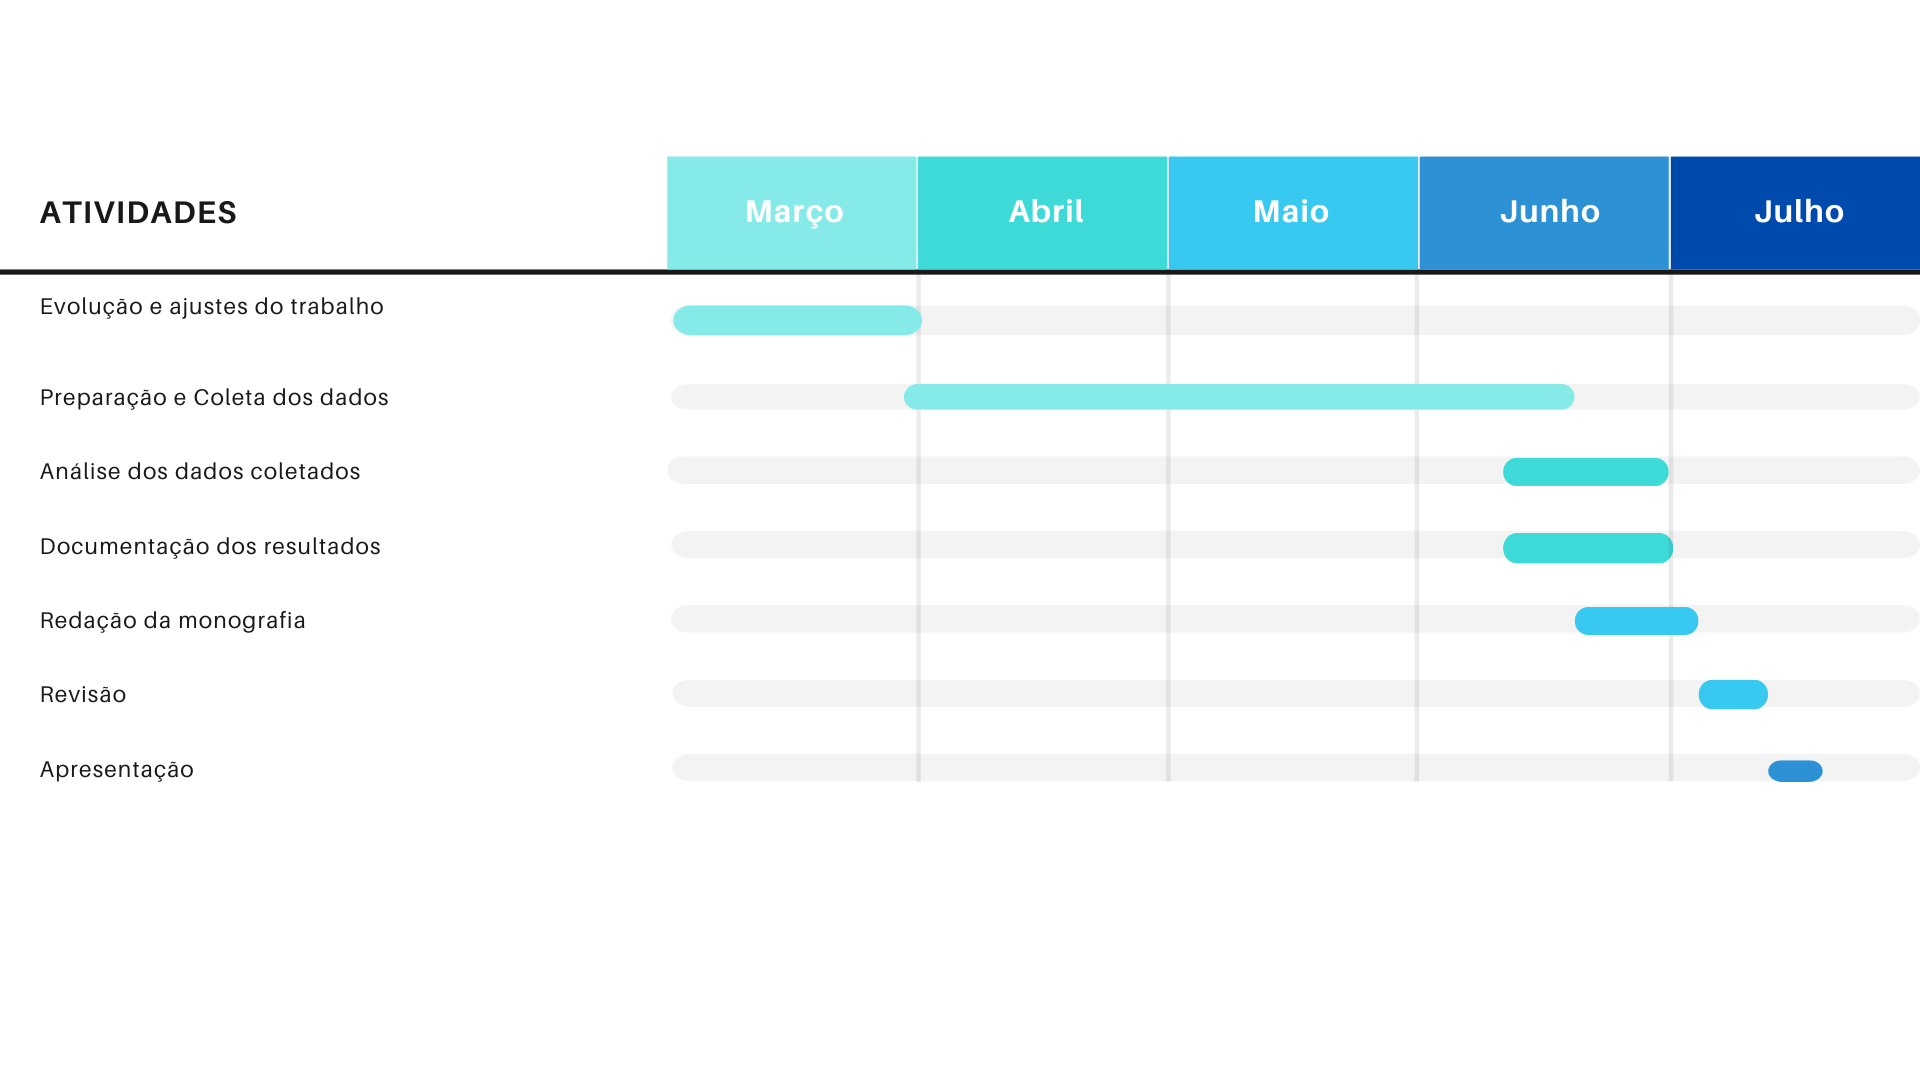
\includegraphics[width=1.1\textwidth]{figuras/Atividades-tcc2-concretizado.png}

    \label{fig:cronograma-atividades-tcc2}
	Fonte: Autor
\end{figure}



\todo[inline, color=pink]{Faltou escrever as subseções das limitações do estudo e trabalhos futuros. Isso é dito na introdução.}

